%----------------------------------------------------------------------------------------
%	PACKAGES & THEMES
%----------------------------------------------------------------------------------------

\documentclass[8pt]{beamer}

\usepackage{etex}
\mode<presentation> {

\usetheme{Vilanova}
}



\usepackage[english]{babel}
\usepackage[utf8]{inputenc}
\usepackage{array}
\usepackage{chronology}
\let\CHRONOLOGY\chronology
\let\endCHRONOLOGY\endchronology
\def\chronology{\shorthandoff{;}\CHRONOLOGY}
\def\endchronology{\endCHRONOLOGY\shorthandon{;}}
\usepackage{pstricks}
\usepackage{graphicx}
\usepackage{booktabs}
\usepackage{amsmath,amssymb,amsthm}
\usepackage{xcolor}
\usepackage{textpos}
\usepackage{tikz}
\usepackage{xmpincl}
\usetikzlibrary{arrows}
\usepackage{pifont}

\usepackage{listings,color}

\definecolor{listcomment}{rgb}{0.0,0.5,0.0}
\definecolor{listkeyword}{rgb}{0.0,0.0,0.5}
\definecolor{listnumbers}{gray}{0.65}
\definecolor{listlightgray}{gray}{0.955}
\definecolor{listwhite}{gray}{1.0}


%% \setbeamertemplate{background canvas}{\includegraphics
%%    [width=\paperwidth,height=\paperheight]{./images/title.pdf}}

\AtBeginSection[]
{
\addtocounter{framenumber}{-1}
\begin{frame}
\frametitle{Outline}
\tableofcontents[currentsection]
\end{frame}}

\newenvironment{shell}
               {\begin{scriptsize}
               \begin{verbatim}}
               {\end{verbatim}\end{scriptsize}}

%----------------------------------------------------------------------------------------
%	PAGE TITRE
%----------------------------------------------------------------------------------------
\title{Land cover mapping with high resolution satellite images using Orfeo Toolbox, QGIS and OSM}
\includexmp{images/cc}
\subtitle{Workshop - W04}
\author{Jordi Inglada (CNES/CESBIO), Julien Michel (CNES), Manuel Grizonnet (CNES)}% date and event here
\date{July 14th 2015 - FOSS4GE, Como, Italy}

\pgfdeclareimage[height=96mm,width=128mm]{background}{../OTB-General/images/fondsClairSansLogo}
\pgfdeclareimage[height=0.2cm]{cc}{../OTB-General/images/CC-licence.png}
\setbeamertemplate{background}{\pgfuseimage{background}}
\pgfdeclareimage[height=0.6cm]{logoIncrust}{../OTB-General/images/logoIncrust}
\logo{
\begin{tabular}{p{0.22\textwidth}p{0.58\textwidth}p{0.1\textwidth}p{0.1\textwidth}}
\href{http://creativecommons.org/licenses/by-sa/3.0/}{\pgfuseimage{cc}}
& \vspace{-0.03\textwidth} \scriptsize{} % date and event here
&  & \href{http://www.orfeo-toolbox.org}{\pgfuseimage{logoIncrust}}\\
\end{tabular}
}

\begin{document}
\begin{frame}
\titlepage
\end{frame}

\section*{Introduction}

\begin{frame}
\frametitle{Disclaimer}

\begin{itemize}
\item We come from the remote sensing world, not the GIS one,
\item What we propose in this workshop works, we tested it! 
\item But ... It may look over-complicated to the GIS ninjas in the audience
\item There are for sure many smarter ways for the GIS processing we will do
\item Not to mention better GIS data sources or more adapted tools!
\item Keep in mind: The workshop focuses on the concept, not the tools (except for Orfeo ToolBox)
\end{itemize}

\end{frame}

\begin{frame}
\frametitle{About land Cover mapping and supervised classification}

\end{frame}

\begin{frame}
\frametitle{Can we use OpenStreetMap as reference data?}



\end{frame}


\begin{frame}
\frametitle{Outline of the workshop}
\begin{block}{In this workshop we will do the following}
\begin{enumerate}
\item Extract relevant data from OpenStreetMap to perform supervised image classification
\item Experiment various classification set-up and assess their performances
\item Use the final classification map to highlight OpenStreetMap shapes that may need an update
\end{enumerate}
\end{block}
\begin{block}{Using the following software}
\begin{itemize}
\item Gdal for vectorial data manipulation
\item Orfeo ToolBox for image processing and classification
\item QGis for visualisation
\end{itemize}
\end{block}
\begin{block}{And data}
\begin{itemize}
\item Spot4Take5 time serie over Ardeche, France as a proxy for future Sentinel2 data,
\item Offline OpenStreetMap export from geofrabrick.de
\end{itemize}
\end{block}

\end{frame}
\section{About the data and software}
\subsection{Data}
\begin{frame}
\frametitle{Spot4Take5 data and upcoming Sentinel 2 data}

\begin{columns}[t]
\begin{column}{5cm}
\begin{block}{Sentinel 2}
\begin{itemize}
\item 2 satellites ESA mission, first launch june 2015
\item Will observe every place on earth every 5 days
\item 13 spectral bands and spatial resolution of 10 to 60 meters
\item Application friendly licence
\end{itemize}
\end{block}
\end{column}
\begin{column}{5cm}
\begin{block}{Spot4Take5}
\begin{itemize}
\item CNES short term experiment for Spot4 end of life
\item Simulate temporal revisit of future S2 mission
\item on 42 sites of 60x60 squared km. around the earth
\item With a spatial resolution of xxx meters and 4 spectral bands
\end{itemize}
\end{block}
\end{column}
\end{columns}

\textcolor{red}{Spot4Take5 data will be used in this workshop as a proxy of future Sentinel 2 data.}

\end{frame}



\begin{frame}
\frametitle{Images overview (Spot4Take5 Ardeche site, France)}

\end{frame}

\begin{frame}
\frametitle{OpenStreetMap data}
\end{frame}

\subsection{Software}
\begin{frame}
\frametitle{The Orfeo ToolBox}
\begin{block}{What is the Orfeo ToolBox?}
\begin{itemize}
\item It is an \textbf{image processing library} dedicated to remote sensing,
\item \textbf{An open-source software} under the CeCILL-v2 licence (french equivalent to GPL),
\item \textbf{Funded by CNES} in the frame of the Orfeo program (and beyond),
\item Written in \textbf{C++} on top of \href{www.itk.org}{ITK} (free medical image processing library),
\item Based on many others image processing and remote sensing open-source software such as Gdal, OSSIM or OpenCV
\item Designed to process large data volume seamlessly thanks to piece-wise processing and multi-threading
\end{itemize}
\end{block}
\begin{center}
{\huge\textcolor{red}{www.orfeo-toolbox.org}}
\end{center}
\end{frame}


\begin{frame}
\frametitle{How to use the Orfeo ToolBox}
\vspace{-0.5cm}
\begin{center}
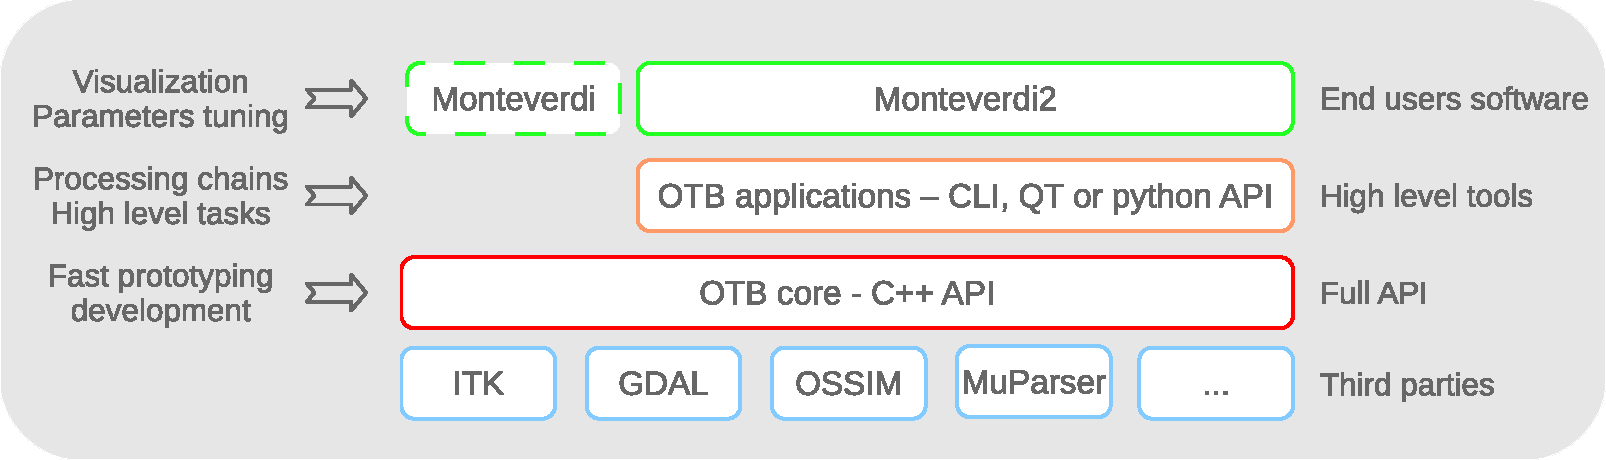
\includegraphics[width=\textwidth]{../OTB-General/images/sandwich.pdf}
\end{center}
\vspace{-0.5cm}
\begin{block}{Write your own code}
 Flexible, Full API available, requires C++ knowledge
\end{block}
\begin{block}{Use OTB applications}
  High level functions (e.g. segmentation), command-line, graphical interface, or python writing availabe. Can be extended (write your own app). Also available in Qgis processing framework.
\end{block}
\begin{block}{Use Monteverdi2}
Data visualization and  \textcolor{red}{access to all applications} in an integrated software
\end{block}
\end{frame}



\begin{frame}
\frametitle{Other software used in this workshop}

\textbf{Do we really need to introduce them ?!?}

\begin{center}
\href{http://gdal.org/}{
\includegraphics[width=0.3\textwidth]{images/gdal.png}} \quad \href{http://qgis.org/en/site/}{
\includegraphics[width=0.3\textwidth]{images/qgis.png}}
\end{center}

We will be using the OSgeoLive 8.5 (Orfeo ToolBox 4.2.1, Gdal 1.11.0, Qgis 2.4.0) USB stick provided by FOSS4GE organization\ldots Time to insert it into your computer! 

\end{frame}


\section{Preparing the data}


\subsection{Image preprocessing}

\begin{frame}
\frametitle{Objectives of this section}

\begin{enumerate}
\item Pre-process image to get it ready for visualisation and classification
\item Learn some basis on command-line OTB processing
\end{enumerate}

\end{frame}


\begin{frame}[fragile]

\frametitle{A first glimpse at the image}

The image is located here :
\begin{scriptsize}
\begin{itemize}
\item Folder: \begin{verbatim}raw_data/spot4t5/SPOT4_HRVIR1_XS_20130607_N2A_CArdecheD0000B0000/\end{verbatim}
\item Image file: \begin{verbatim}SPOT4_HRVIR1_XS_20130607_N2A_ORTHO_SURF_CORR_PENTE_CArdecheD0000B0000.TIF\end{verbatim}
\end{itemize}
\end{scriptsize}

\begin{enumerate}
\item Open the image in Qgis
\item In layer properties:
  \begin{enumerate}
    \item Set the no data value to -10 000 in the transparancy tab,
    \item In the style tab, change color composition to r=b3,g=b2,b=b1,
    \item Reload statistics in the Style tab.
  \end{enumerate}
\end{enumerate}
What do you see ?
\end{frame}

\begin{frame}
\frametitle{Natural colors synthesis} 
Spot4 images have the following spectral bands: Green (b1), Red (b2), Near Infra-Red (b3), Short Wavelength Infra-Red (b4)

To get familiar with Orfeo ToolBox processing, and to ease data
visualisation, we will build a synthetic green and blue channel with the following formula:

\begin{equation}
b=0.7*green+0.24*red-0.14*swir
\end{equation}
We are going to use the BandMath application, as well as the ConcatenateImages application.

\textcolor{red}{Caution: this synthetic image is only for visualisation, not for processing!}

\end{frame}
\begin{frame}[fragile]
\frametitle{Natural colors synthetis (Solution)}
Extract red band:
\begin{verbatim}
$ otbcli_BandMath -il im.tif -out red.tif int16 -exp "im1b2"
\end{verbatim}
Extract green band:
\begin{verbatim}
$ otbcli_BandMath -il im.tif -out green.tif int16 -exp "im1b1"
\end{verbatim}
Compute synthetic blue band:
\begin{verbatim}
$ otbcli_BandMath -il im.tif -out blue.tif int16 \
 -exp "im1b1==-10000?-10000:0.7*im1b1+0.24*im1b2-0.14*im1b3"
\end{verbatim}
Concatenate all bands:
\begin{verbatim}
$ otbcli_ConcatenateImages -il red.tif green.tif blue.tif -out rgb.tif int16
\end{verbatim}

Open resulting image in qgis, and set the rendering option likewise.

\end{frame}

\begin{frame}[fragile]
\frametitle{Radiometric indices that help classification}

We will compute two more things that will help the classification process:
\begin{itemize}
\item A Normalize Difference Vegetation Index:
\begin{equation}
ndvi = (nir-red)/(nir+red)
\end{equation}
\item A Normalize Difference Water Index:
\begin{equation}
ndvi = (nir-swir)/(nir+swir)
\end{equation}
You can visualize the result in qgis, and concatenate these two bands with the original image
\end{itemize}

\begin{block}{Solution}
\begin{scriptsize}
\begin{verbatim}
$ otbcli_BandMath -il im.tif -out ndvi.tif int16 -exp "im1b1==-10000?-10000:(im1b3-im1b2)/(im1b3+im1b2)"
\end{verbatim}
\end{scriptsize}
\begin{scriptsize}
\begin{verbatim}
$ otbcli_BandMath -il im.tif -out ndwi.tif int16 -exp "im1b1==-10000?-10000:(im1b3-im1b4)/(im1b3+im1b4)"
\end{verbatim}
\end{scriptsize}
\begin{scriptsize}
\begin{verbatim}
$ otbcli_ConcatenateImages -il im.tif ndvi.tif ndwi.tif -out im4classif.tif
\end{verbatim}
\end{scriptsize}
\end{block}
\end{frame}

\subsection{OpenStreetMap preprocessing}

\begin{frame}
\frametitle{Objectives of this section}

\begin{enumerate}
\item Turn OSM data into a vector layer suitable for classifier training:
\begin{enumerate}
\item Filter and join features to get a limited number of well-defined classes (in the sense of classification)
\item Build a single layer with polygon feature bearing an integer class attribute
\end{enumerate}
\item Learn how training polygons should be and which features of OSM are suitable
\end{enumerate}

\end{frame}


\begin{frame}[fragile]
\frametitle{Pre-processing OpenStreetMap data}

For each region, open the following files on top of the image in Qgis:
\begin{itemize}
\item \begin{verbatim}landuse.hsp\end{verbatim}
\item \begin{verbatim}natural.hsp\end{verbatim}
\item \begin{verbatim}waterways.hsp\end{verbatim}
\end{itemize}

To get OpenStreetMap data ready for classification, we will do the following:
\begin{enumerate}
\item Extract geometries that actually cover our image (area of interest)
\item Reproject all geometries in the image SRS
\item Filter OSM classes to build a set of 3 classes suitable for supervised classification
\item Process waterways to turn polylines into polygons with buffers
\item Randomly extract a limited number of features for each class.
\end{enumerate}
\end{frame}

\begin{frame}[fragile]
\frametitle{Extracting geometries that cover our image}
\begin{block}{Extracting image footprint}
% Alternative: dessiner une enveloppe plus précise à la main (à cause du no-data)
\begin{enumerate}
\item Use the ImageEnvelope application
\item Output a shapefile or sqlite file
\item Control results in Qgis
\end{enumerate}
\end{block}

\begin{block}{Clip OSM layers to ROI and reproject to image SRS}
\begin{enumerate}
\item For each region and each layer
\item Use \texttt{ogr2ogr}
\item Use the \texttt{-clipsrc} option to filter by image footprint
\item Use the \texttt{-t\_srs} option to define the output SRS using the \texttt{l93.wkt} file
\item Use the \texttt{-append} option to merge both regions for each layer
\end{enumerate}
\end{block}

\end{frame}

\begin{frame}[fragile]
\frametitle{Extracting geometries that cover our image (solution)}
Extract image enveloppe:
\begin{scriptsize}
\begin{verbatim}
$ otbcli_ImageEnvelope -in SPOT4_HRVIR1_XS_20130607_rgb.tif -proj "EPSG:32631" -out env.shp
\end{verbatim}
\end{scriptsize}
Clipping, reprojecting and merging land use layers:
\begin{scriptsize}
\begin{verbatim}
$ ogr2ogr -append -t_srs raw_data/l93.wkt -clipsrc env.shp landuse_l93.shp raw_data/osm/auvergne/landuse.shp
$ ogr2ogr -append -t_srs raw_data/l93.wkt -clipsrc env.shp landuse_l93.shp raw_data/osm/rhone-alpes/landuse.shp
\end{verbatim}
\end{scriptsize}
Clipping, reprojecting and merging natural layers:
\begin{scriptsize}
\begin{verbatim}
$ ogr2ogr -append -t_srs raw_data/l93.wkt -clipsrc env.shp natural_l93.shp raw_data/osm/auvergne/natural.shp
$ ogr2ogr -append -t_srs raw_data/l93.wkt -clipsrc env.shp natural_l93.shp raw_data/osm/rhone-alpes/natural.shp
\end{verbatim}
\end{scriptsize}
Clipping, reprojecting and merging waterways layers:
\begin{scriptsize}
\begin{verbatim}
$ ogr2ogr -append -t_srs raw_data/l93.wkt -clipsrc env.shp waterways_l93.shp raw_data/osm/auvergne/waterways.shp
$ ogr2ogr -append -t_srs raw_data/l93.wkt -clipsrc env.shp waterways_l93.shp raw_data/osm/rhone-alpes/waterways.shp
\end{verbatim}
\end{scriptsize}

Open the three new layers in Qgis.
\end{frame}

\begin{frame}[fragile]
\frametitle{Build consistent classes for supervised classification}
\begin{block}{The idea}
\begin{itemize}
\item Select and join OSM features from landuse and natural layers
\item That form simple landcover classes (e.g. water or vegetation)
\item Which are big enough wrt. to image resolution (20m)
\item You can walk the layers and have a look at OSM spec here\footnote{\url{https://wiki.openstreetmap.org/wiki/Map_Features}}
\end{itemize}
\end{block}

\begin{block}{Our Proposal}
\begin{itemize}
\item \textbf{Water:} 
  \begin{itemize}
  \item basin, pond, reservoir, salt pond, water, wetland larger than 1000 squared meters from land use layer
  \item water larger than 1000 squared meters from natural layer
  \item main rivers (Loire, Rhone) from waterways layer, buffered with 25 meters
  \end{itemize}
\item \textbf{Vegetation:} forest from natural layer
\item \textbf{Built-up:} residential, commercial, cemetery, construction, industrial, recreational, harbour, allotments, yard, brownfield, vine from land use layer
\end{itemize}
\end{block}

\end{frame}

\begin{frame}[fragile]
\frametitle{Building the water class}
\begin{enumerate}
\item Extract the two large rivers covering the image:
\begin{scriptsize}
\begin{verbatim}
$ ogr2ogr -append -sql "select * from waterways_l93 where name in \
  ("La Loire", "Le Rhone")" large_rivers.shp waterways_l93.shp
\end{verbatim}
\end{scriptsize}

\item In Qgis, use the \textit{vector/geoprocessing/buffer} tool to build a 25m buffer around, and save it to \texttt{water.shp}.

\item Append selected features from land use layer:
\begin{scriptsize}
\begin{verbatim}
$ ogr2ogr -append -sql "select * from landuse_l93 where type in \ 
  (\"basin\",\"pond\",\"reservoir\",\"salt_pond\",\"water\",\"wetland\") \
  and OGR_GEOM_AREA > 10000" water.shp landuse_l93.shp
\end{verbatim}
\end{scriptsize}

\item Append selected features from natural layer:
\begin{scriptsize}
\begin{verbatim}
$ ogr2ogr -append -sql "select * from natural_l93 where type in \
  (\"water\") and OGR_GEOM_AREA > 1000" water.shp natural_l93.shp
\end{verbatim}
\end{scriptsize}
\end{enumerate}
\end{frame}

\begin{frame}[fragile]
\frametitle{Building the vegetation and built-up classes}
\begin{block}{Vegetation class}
Extract selected features from natural layer:
\begin{scriptsize}
\begin{verbatim}
$ ogr2ogr -append -sql "select * from natural_l93 where type in \
  (\"forest\")" forest.shp natural_l93.shp
\end{verbatim}
\end{scriptsize}
\end{block}

\begin{block}{Built-up class}
Extract selected features from land use layer:
\begin{scriptsize}
\begin{verbatim}
$ ogr2ogr -append -sql "select * from landuse_l93 where type in \
  (\"residential\",\"commercial\",\"cemetery\",\"construction\",\
  \"industrial\",\"résidential\",\"recreational\",\"harbour\",  \
  \"allotments\",\"vineyard\",\"brownfield\")" builtup.shp landuse_l93.shp
\end{verbatim}
\end{scriptsize}
\end{block}
\end{frame}

\begin{frame}[fragile]
\frametitle{Final step: add class label and merge in one layer}

\begin{block}{Add class labels}
\begin{itemize}
\item Goal: create a new integer field with a unique id for each of the 3 classes
\item Can be done in Qgis attribute table manager
\item Or With the VectorDataSetField application in OTB
\end{itemize}
\end{block}

\begin{block}{Merge all layers}
\begin{scriptsize}
\begin{verbatim}
$ ogr2ogr -append training_set.shp water.shp
$ ogr2ogr -append training_set.shp forest.shp
$ ogr2ogr -append training_set.shp builtup.shp
\end{verbatim}
\end{scriptsize}
\end{block}

You can display the final training layer in Qgis with a color mapping of classes.
\end{frame}

\section{Image Classification}

\begin{frame}
\frametitle{Objectives of this section}

\begin{enumerate}
\item Learn the steps of supervised classification processing with Orfeo ToolBox
\item Perform the classification based on the OSM pre-processed data
\end{enumerate}

\end{frame}

\subsection{Estimation of image statistics}

\begin{frame}
\frametitle{Step 1: Estimation of image statistics}

\begin{itemize}
\item Some machine learning algorithm requires the input features to have similar ranges
\item Also, the SVM algorithm will converge faster if this range is $[-1,1]$
\item We will therefore center and reduce all image bands prior to classification
\item For this, we need to estimate the mean and variance of each band
\item Which is what this step is about
\end{itemize}

For this we will use the \texttt{EstimateImagesStatistics} application. Do not forget to set the background value (-10 000)!

\end{frame}

\begin{frame}[fragile]
\frametitle{Step 1: Estimation of image statistics (solution)}

\begin{scriptsize}
\begin{verbatim}
$ otbcli_ComputeImagesStatistics -il im4classif.tif -out stats.xml -bv -10000
\end{verbatim}
\end{scriptsize}

Look  at the \texttt{stats.xml} file. Does it look correct?

\end{frame}

\subsection{Training of the classification algorithm}

\begin{frame}
\frametitle{Step 2: Training the classification algorithm}

\begin{itemize}
\item We will be using the \texttt{TrainImagesClassifier} application
\item The application should receive the image, the training layer and the xml stats file,
\item We will use the libsvm implementation, with a RBF kernel,
\item We will select at most 1000 random samples per class (2000 for validation),
\item You also need to set the name of the class field in the training layer.
\end{itemize}


\end{frame}


\begin{frame}[fragile]
\frametitle{Step 2: Training the classification algorithm (solution)}

\begin{scriptsize}
\begin{verbatim}
$ otbcli_TrainImagesClassifier -io.il im4classif.tif -io.vd training_set.shp -io.out model.svm \
  -classifier libsvm -classifier.libsvm.k rbf -sample.mt 1000  -sample.mv 2000 \
  -sample.vfn "class" -io.imstat stats.xml

...

2015 Jun 12 14:25:29  :  Application.logger  (INFO) Confusion matrix (rows = reference labels, columns = produced labels):
     [1] [2] [3] 
[ 1] 1609  190  178 
[ 2]   84 1698  211 
[ 3]   60  148 1771 

2015 Jun 12 14:25:29  :  Application.logger  (INFO) Precision of class [1] vs all: 0.917855
2015 Jun 12 14:25:29  :  Application.logger  (INFO) Recall of class    [1] vs all: 0.813859
2015 Jun 12 14:25:29  :  Application.logger  (INFO) F-score of class   [1] vs all: 0.862735

2015 Jun 12 14:25:29  :  Application.logger  (INFO) Precision of class [2] vs all: 0.833988
2015 Jun 12 14:25:29  :  Application.logger  (INFO) Recall of class    [2] vs all: 0.851982
2015 Jun 12 14:25:29  :  Application.logger  (INFO) F-score of class   [2] vs all: 0.842889

2015 Jun 12 14:25:29  :  Application.logger  (INFO) Precision of class [3] vs all: 0.819907
2015 Jun 12 14:25:29  :  Application.logger  (INFO) Recall of class    [3] vs all: 0.894896
2015 Jun 12 14:25:29  :  Application.logger  (INFO) F-score of class   [3] vs all: 0.855762

\end{verbatim}
\end{scriptsize}

\end{frame}

\subsection{Classifying the image}

\begin{frame}
\frametitle{Step 3: Classifying the image}

\begin{itemize}
\item Now that we trained a classifier with a satisfactory level of performance, lets classify the image,
\item We will use the \texttt{ImageClassifier} application,
\item It should receive the input image, the model and the stats files,
\item We will also build a mask of no data pixels, so that they will be ignored during classification (use the \texttt{BandMath} app for this)
\end{itemize}

\end{frame}


\begin{frame}[fragile]
\frametitle{Step 3: Classifying the image (solution)}

\begin{scriptsize}
\begin{verbatim}
$ otbcli_BandMath -il im4classif.tif -out mask.tif uint8 -exp "im1b1>-10000?255:0"
$ otbcli_ImageClassifier -in im4classif.tif -mask mask.tif -model model.svm -imstat stats.xml -out classif.tif uint8
\end{verbatim}
\end{scriptsize}
Open the resulting land cover map in Qgis. Set the rendering to color each class with a discriminative color. Does the classification map look correct?
\end{frame}


\subsection{Noise cleaning}

\begin{frame}
\frametitle{Step 4: Classification noise cleaning}

\begin{itemize}
\item Classification maps often suffer from salt and pepper noise (isolated pixels with class different from neighborhood)
\item We can filter that with the \texttt{ClassificationMapRegularization} application
\item It will perform a majority voting of classified pixels in a fixed neighborhood (radius = 2 for instance)
\end{itemize}

\end{frame}

\begin{frame}[fragile]
\frametitle{Step 4: Classification noise cleaning}
\begin{scriptsize}
\begin{verbatim}
$ otbcli_ClassificationMapRegularization -io.in classif.tif -io.out classif_reg.tif -ip.radius 2
\end{verbatim}
\end{scriptsize}

Load the cleaned map into QGis as well.

\end{frame}

% Add a step to estimate the final accuracy ?

\section{Getting back to OpenStreetMap}



\end{document}
